\section{Definierte und bestehende Prozesse (Regelung und Handhabung von vorhandenen Informationen)}

\subsection{Wissensmanagement}
Wissensmanagement ist für die Hochschule Emden/Leer ein sehr wichtiger Aspekt, da Sie täglich mit dem Erwerb, der Entwicklung, dem Transfer sowie der Nutzung von Wissen konfrontiert wird. Für den Betrieb eines erfolgreichen Wissensmanagements ist an ein klares Regelwerk die Voraussetzung.

\subsection{E-Learning}
\todo{Quellenangabe?}
Laut Michael Kerres\footnote{Ich bin eine Quelle, bezeichne mich} ist E-Learning das Lehren und Lernen bei dem elektronische Medien für die Präsentation und Distribution von Lehrmaterialien und Kommunikation zum Einsatz kommen.

\subsubsection{E-Learning an der Hochschule Emden/Leer}
E-Learning ist an der Hochschule Emden/Leer ein sehr wichtiges Thema, da an der Hochschule der Studiengang Medieninformatik (Online), Wirtschaftsinformatik (Online) akkreditiert  wurde. Nun soll dargelegt werden ob in den Präsenzstudiengängen ebenfalls das Thema E-Learning Einzug gehalten hat.

\subsubsection{E-Learning in den Präsenzstudiengängen}
Es soll betrachtet werden in welchen Präsenzstudiengängen E-Learning eingesetzt wird.

\missingfigure{Grafik E-Learning Präsenzstudium}

Aus der Grafik geht hervor, dass der Fachbereich SAG (Soziale Arbeit und Gesundheit) der Vorreiter aller Fachbereiche mit der Einführung eines E-Learning Systems war. SAG setzt mehr als 200 Onlinekurse im Präsenzstudium ein. Auch für die Anmeldung an verschiedenen Kursen kommt ein Online-System zum Einsatz.

Es folgt dann der Fachbereich Technik in dem E-Learning ebenfalls sehr stark verbreitet ist, da die Studiengänge Medieninformatik und Wirtschaftsinformatik als reine Onlinestudiengänge in diesem etabliert sind.

Weniger stark wird E-Learning vom Fachbereich Wirtschaft betrieben. Das geringste Nutzungsverhalten ist im Fachbereich Seefahrt zu verzeichnen.

Trotz des unterschiedlichen Nutzungsverhaltens hat E-Learning in allen Fachbereich Einzug gehalten.

\subsubsection[Einsatz von E-Learning-Anwendungen]{Einsatz von E-Learning-Anwendungen in den Präsenzstudiengängen}
Im diesem Abschnitt wird erläutert, ob die Anwendungen Adobe Connect, Moodle im Präsenzstudiengang eingesetzt werden.

\paragraph{Adobe Connect}
Adobe Connect ist eine Kommunikationsplattform zur Bereitstellung von Webmeetings und E-Learning-Inhalten.

Ausschließlich der Fachbereich Technik (E+I) nutzt durch seine Onlinestudiengänge die Plattform Adobe Connect als Medium des visuellen Austausches von Bild und Sprache. In den Präsenzstudiengängen kommt die Plattform nicht zum Einsatz, da der persönliche Austausch von Studierenden und Dozenten in den täglichen Präsenzen stattfindet.

\paragraph{Moodle}
Die Hochschule Emden/Leer setzt Moodle als Lernplattform ein. Moodle ist ein freies objektorientiertes Kursmanagementsystem welches prädestiniert ist für den Einsatz von E-Learning Inhalten.\footnote{\url{https://moodle.hs-emden-leer.de/moodle/}}

\begin{figure}[h!]
	\centering
	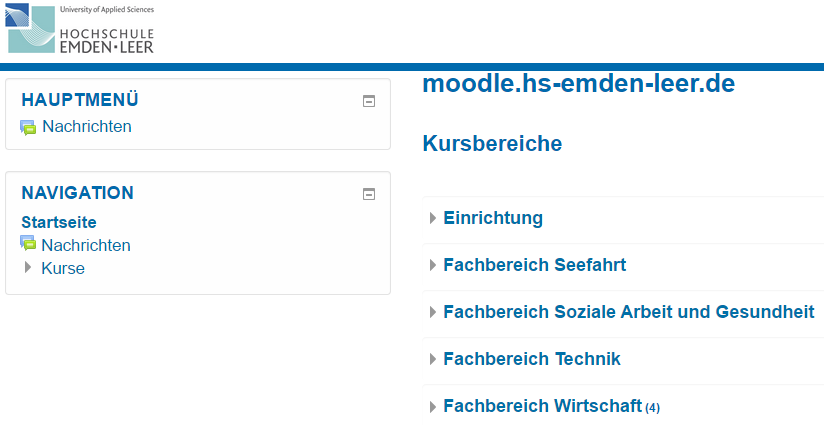
\includegraphics[width=8cm]{kapitel/gruppe2/bilder/moodle}
	\caption{Übersicht Moodle für alle}
	\label{fig_moodle}
\end{figure}

Durch den Einsatz von Moodle in allen Fachbereichen, wird das volle Leistungsspektrum des Systems ausgenutzt. Folgende Funktionalitäten werden angeboten:
\begin{itemize}
	\item Lernvideos
	\item Vorlesungsskripte
	\item Forum
	\item Kalender
	\item Mail-Connect
\end{itemize}

Für jeden Fachbereich wird der volle Funktionsumfang der Plattform zur Verfügung gestellt, auch wenn nicht jeder Fachbereich jeden Service nutzt.

\subsubsection{Zentrale Informationsbereitstellung durch Datenlaufwerke}
Für alle beteiligten der Hochschule Emden/Leer werden spezielle Datenlaufwerke zur Verfügung gestellt. Es handelt sich um 3 Netzlaufwerke auf den Fileservern der Hochschule.\footnote{\url{https://connect.hs-emden-leer.de/cgi-bin/portal}}

\begin{figure}[h!]
	\centering
	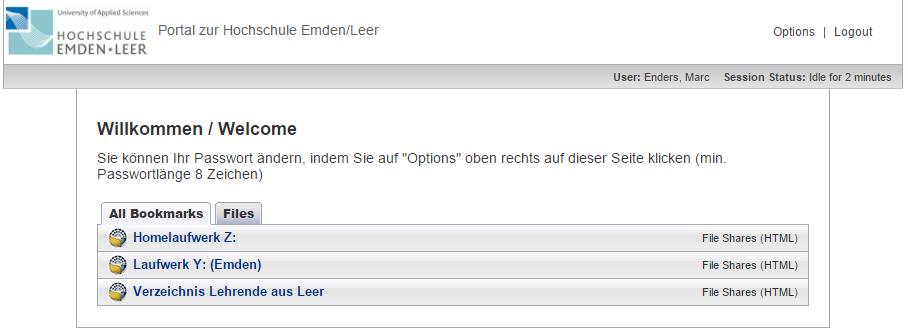
\includegraphics[width=8cm]{kapitel/gruppe2/bilder/zugriff_auf_laufwerke_extern}
	\caption{Zugriff auf die Datenlaufwerke von extern}
	\label{fig_zugriff_datenlaufwerke_extern}
\end{figure}


\paragraph{Laufwerk Z}
Auf dem Laufwerk Z befinden sich die Daten des Home-Verzeichnisses jedes einzelnen Benutzers. Meldet sich dieser an beliebigen Rechnern des Rechnerpools an, werden die Inhalte Ihres Home-Verzeichnisses automatisch eingebunden. Der interne Zugriff auf die eigenen Dateien ist von jedem Rechner des Pools möglich, da servergespeicherte Profile zum Einsatz kommen. Auch von externe können die Studierenden problemlos auf die Ressourcen der Datenlaufwerke zugreifen.

\paragraph{Laufwerk Y}
Für den gemeinsamen Austausch der Daten wurde das Transferlaufwerk Y eingerichtet. Hier werden zentral Ressourcen für alle Studierenden und Lehrenden aus Emden zum Austausch zur Verfügung gestellt.

\paragraph{Verzeichnis Lehrende aus Leer}
Zusätzlich zum Transferlaufwerk steht das Verzeichnis der Lehrenden aus Leer  zur Verfügung. Hier stellen die Lehrenden Inhalte zur Verfügung.

\subsubsection{Moodle vs. Datenlaufwerke für Präsenzstudenten}
An der Moodle-Plattform melden sich die Nutzer über eine webbasierte Oberfläche am System an. Um Dateien zur Verfügung zu stellen, muss auf der Weboberfläche zu den gewünschten Reitern navigiert werden.

Stellt man die Datenlaufwerke (Y Laufwerk und Transferlaufwerk der Lehrenden) der Moodle-Plattform gegenüber  und betrachtet nur den Aspekt des Datenaustausches, so wird deutlich, dass der Dateiaustausch über   Datenlaufwerke in Bezug auf Komfort und Aufwand deutlich besser für die Präsenzstudierenden geeignet ist, als die Dateiablage über die Moodle-Plattform. Die über die Datenlaufwerke zur Verfügung gestellten Inhalte können von den Studierenden mit wenig Aufwand intuitiv erreicht werden.

Aus dem Interview mit dem Rechenzentrumsleiter Herrn Günter Müller kristallisierte sich heraus, dass der Fachbereich Wirtschaft die Datenlaufwerke am stärksten und der Fachbereich Technik und andere Fachbereiche diese weniger stark nutzen.

\subsection{Sicherheitsaspekte}
(\ldots)

\subsubsection{Sicherheitsrichtlinien an der Hochschule Emden / Leer}
Der Einsatz von Sicherheitsrichtlinien ist ein wichtiges Thema an Hochschulen. Sicherheitsrichtlinien beschreiben die Sicherstellung von Verfügbarkeit, Integrität, Vertraulichkeit und Authentizität von Informationen.

An der Hochschule Emden/Leer werden als Basis für die Informationssicherheit Teile des IT-Grundschutz-Kataloges umgesetzt. Nicht alle Empfehlungen des BSI sind an einer kleinen Hochschule, wie die Hochschule Emden/Leer es ist, umsetzbar.

An den Serverräumen der Hochschule ist die Umsetzung der IT-Grundschutzmaßnahmen deutlich zu erkennen.

Folgende physikalische Schutzmaßnahmen wurden an der Hochschule Emden/Leer in den Serverräumen umgesetzt:

\begin{itemize}
	\item einbruchsicher
	\item feuergemeldet
	\item videoüberwacht
	\item Lage der Serverräume im 1. OG (Wasserschutz)
\end{itemize}

\subsubsection{Einsatz von ITIL}
Die IT Infrastructure Libary (ITIL) ist eine Sammlung von Best Practises zur Umsetzung eines IT-Service-Managements (ITSM). In diesem Regelwerk werden die für den Betrieb einer IT-Infrastruktur notwendigen Prozesse und Werkzeuge beschrieben.
Der ITIL-Prozess ist an der Hochschule Emden/ Leer nicht etabliert, da die Personaldecke für die Umsetzung eines 1st und 2nd-Level Supports nicht gegeben ist.\footnote{\url{http://de.wikipedia.org/wiki/IT_Infrastructure_Library}}

\subsubsection{Umsetzung von ISO/IEC 27001}
Die ISO/IEC 27001 Zertifizierung wird auf Basis des IT-Grundschutzes vergeben. Durch die Zertifizierung des ISO/IEC 27001 Standards haben Unternehmen, Behörden, Organisationen die Möglichkeit, ihre Bemühungen um Informationssicherheit nach innen und außen zu dokumentieren.

Das Einsatzszenario ist an der Hochschule Emden/Leer nicht gegeben, da für Umsetzung die Personaldichte zu gering ist. Für die Erfüllung der Zertifizierung würde riesiger Personaloverhead entstehen.\footnote{\url{https://www.bsi.bund.de/DE/Themen/ZertifizierungundAnerkennung/Zertifizierung27001/GS_Zertifizierung_node.html}}

\subsubsection{Single Sign-On}
(\ldots)

\subsubsection{Fazit Sicherheitsrichtlinien}
Abschließend ist zu sagen, dass an der Hochschule Emden/Leer der IT-Sicherheitsaspekt ein sehr wichtiges Thema ist. Als kleine Hochschule ist es auf Grund der Personaldichte nicht möglich, alle Empfehlungen des BSI-Grundschutzes, ITIL und ISO/IEC 27001 umzusetzen. Jedoch sucht sich die Hochschule aus den Regelwerken die Empfehlungen heraus, die auf Grund der Personaldichte umsetzbar sind.  Dies bildet eine sehr gute Basis im Hinblick auf das sehr anspruchsvolle Thema IT-Sicherheit.


